\section{Auswertung}
\label{sec:Auswertung}

Die Graphen werden sowohl mit Matplotlib \cite{matplotlib} als auch NumPy \cite{numpy} erstellt. Die Fehlerrechnung wird mithilfe von Uncertainties \cite{uncertainties} durchgeführt. Die Naturkonstanten werden dem Paket Scipy \cite{scipy} entnommen.
In Tabelle \ref{tab:values} befinden sich Materialspezifische Werte, die für spätere Rechnungen benötigt werden.

\begin{table}
	\centering
	\caption{Die Kernladungszahl $Z$, die Dicke der Folie $d$, die Teilchendichte $n=\frac{\rho}{m}$ für Gold, Aluminium und Bismut \cite{Elemente16}.}
	\label{tab:tabZWerte}
	\sisetup{table-format=1.2}
	\begin{tabular}{lS[table-format=2.0]S[table-format=1.0]S[table-format=1.1]}
		\toprule
		{Element} & {$Z$} & {$d/\si{\micro\metre}$} & {$n/10^{28}\si{\metre^{-3}}$} \\
		\midrule
		{Gold} & 79 & 2 & 5.9  \\
		{Aluminium} & 13 & 3 & 6.2  \\
		{Bismut} & 83 & 1 & 2.9  \\
		\bottomrule
	\end{tabular}

	\label{tab:values}
\end{table}

\subsection{Bestimmung der Aktivität}

Die Aktivität der Probe wird über das Zerfallsgesetz, sowie über eine Nullmessung bestimmt.
Mit dem Zerfallsgesetz bestimmt sich die Aktivität über: 
\[
A = A_0 .e^{-\frac{\ln(2)}{\tau}t}\text{.}
\]
Dabei entspricht $A_0 = \SI{330(1)}{\kilo\becquerel}$ \cite{V16} der Aktivität der Probe im Oktober 1994, $\tau = \SI{432.6(6)}{\second}$ \cite{Americium} der Halbwertszeit für $^{241}.{Am}$ und $t = \SI{7,665(13)e8}{\second}$ der seit Oktober 1994 vergangenen Zeit. Es ergibt sich:
\[
A_.{theo} = \SI{317.4(10)}{\kilo\becquerel} \text{.}
\]
Der Fehler $\sigma_{A_.{theo}}$ ergibt sich dabei aus dem Fehler auf $A_0$, da dieser überwiegt.
Bei der $t = \SI{300}{\second}$ langen Nullmessung im Vakuum von $\SI{0,033}{\milli\bar}$ und ohne Folie wurden $N = \num{4539(68)}$ Teilchen registriert. Der Fehler $\sigma_N=\sqrt{N}$ entsteht durch die Poisson-Verteilung. 
Damit ergibt sich die Aktivität pro Raumwinkelelement zu:
\[
\frac{\Omega A_.{exp}}{4\pi} = \frac{N}{t} = \SI{15,13(22)}{\becquerel} \text{.}
\] 
Der Fehler $\sigma_{A_.{exp}}=\frac{\sigma_N}{t}$ folgt aus der Gaußschen Fehlerfortpflanzung. 
Das Raumwinkelelement $\frac{\Omega}{4\pi}$ bestimmt sich aus dem Verhältnis der vom Detektor abgedeckten Fläche zur Oberfläche einer Kugel, deren Radius $r = \SI{101}{\milli\metre}$ \cite{V16} dem Abstand der Quelle zum Detektor entspricht. Die abgedeckte Fläche wird wegen der Kollimation der $\SI{2}{\milli\metre}$ Schlitzblenden zu $\SI{4}{\milli\metre\squared}$ genähert. Der tatsächliche Wert ist als größer anzunehmen, weswegen eine zu große Aktivität zu erwarten ist. Es ergibt sich:
\[
\frac{\Omega}{4\pi} = \num{3,12e-5}\text{.}
\]   
Daraus folgt für die Aktivität:
\[
A_.{exp} = \SI{485(7)}{\kilo\becquerel} \text{.}
\]

\subsection{Form der vorverstärkten Impulse auf dem Oszilloskop}

Es werden die vorverstärkten Impulse einmal mit und einmal ohne Amplifier betrachtet. Die Bilder sind in den Abbildungen \ref{fig:ohneAmplifier} und \ref{fig:mitAmplifier} zu sehen. Dabei ist die Spannung gegen die Zeit aufgetragen. In beiden Fällen ist ein Untergrundrauschen erkennbar.\\
Ohne Amplifier steigt die Spannung sprunghaft auf einen Maximalwert von $\SI{140}{\milli\volt}$ an und fällt dann exponentiell in die Ruhelage zurück.
Mit Amplifier ist eine Anstiegszeit von $\SI{1}{\micro\second}$ auf ein Maximum von $\SI{4,5}{\volt}$ zu erkennen. Die Kurve nimmt einen Gaußförmigen verlauf an, wobei die linke Flanke steiler ist als die Rechte.\\

\begin{figure}
	\centering
	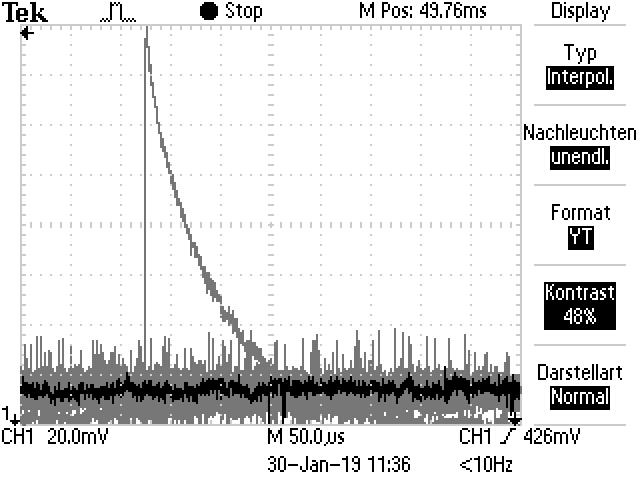
\includegraphics[width=\linewidth-60pt,keepaspectratio]{content/images/ohneVerstaerker02.jpg}
	\caption{Der Impulsverlauf am Oszilloskop ohne Amplifier.}
	\label{fig:ohneAmplifier}
\end{figure}

\begin{figure}
	\centering
	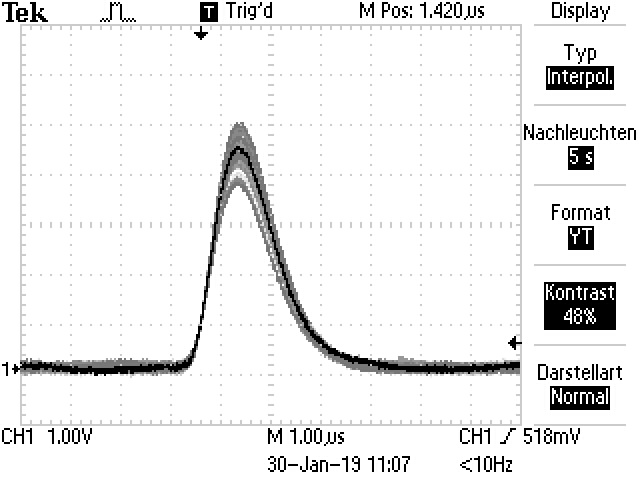
\includegraphics[width=\linewidth-60pt,keepaspectratio]{content/images/mitVerstaerker01.jpg}
	\caption{Der Impulsverlauf am Oszilloskop mit Amplifier.}
	\label{fig:mitAmplifier}
\end{figure}

\subsection{Bestimmung der Foliendicke mittels einer Energieverlustmessung}

Durch eine Energieverlustmessung wird die Dicke einer Goldfolie bestimmt. Dazu wird einmal mit und einmal ohne Folie die Spannung $U$ der Impulse bei verschiedenen Drücken $p$ gemessen. Da die Impulshöhe schwankt, wird der Mittelwert aus der unteren Grenze, der oberen Grenze und dem vermuteten Mittel mit der Formel für den Mittelwert
\[
\mu_U = \frac{1}{N}\sum_{i=1}^N U_i
\]
und dessen Standardabweichung
\[
\sigma_U = \sqrt{\frac{1}{N(N-1)}\sum_{i=1}^N (U_i-\mu_U)^2}
\]
gebildet zu
\[
U = \mu_U \pm \sigma_U \text{.}
\]
Die Werte befinden sich in den Tabellen \ref{tab:dataOhne} und \ref{tab:dataMit}. Die Graphen sind in Abbildung \ref{fig:Foliendicke} zu sehen.
Es werden lineare Ausgleichsrechnungen der Form
\[
U = ap + b
\]
durchgeführt. Dies ergibt die Parameter:
\begin{align*}
a_.{ohne} &= \SI{-1.213(20)e-2}{\volt\per\milli\per\bar}\\
b_.{ohne} &= \SI{4.372(18)}{\milli\bar}\\
a_.{mit}  &= \SI{-1.38(7)e-2}{\volt\per\milli\per\bar}\\
b_.{mit}  &= \SI{3.47(6)}{\milli\bar}\text{.}
\end{align*}
Die Parameter $a_.{ohne}$ und $b_.{ohne}$ gehören dabei zur Messung ohne Folie, die Parameter $a_.{mit}$ und $b_.{mit}$ zu der mit Folie.
Der Energieverlust lässt sich mit Formel \eqref{eq:dx} aus den Achsenabschnitten $b_.{ohne}$ und $b_.{mit}$ bestimmen. Dazu muss ein Umrechnungsfaktor $\kappa$ von der Spannung in die Energie bestimmt werden. Aus der Theorie ist mit $E_\alpha=\SI{5,486}{\mega\electronvolt}$ die Energie der $\alpha$-Teilchen im Vakuum bekannt. Es ergibt sich:
\[
\kappa = \frac{E_\alpha}{b_.{ohne}} = \SI{1.255(5)}{\mega\electronvolt\per\volt}\text{.}
\]
Der Fehler $\sigma_\kappa$ bestimmt sich nach der Gaußschen Fehlerfortpflanzung:
\[
\sigma_\kappa = \frac{E_\alpha}{b_.{ohne}}\sigma_{b_.{ohne}}\text{.}
\]
%Der Energieverlust lässt sich über die Spannungsdifferenz der y-Achsenabschnitte bestimmen, indem die Proportionalität zur Energie genutzt wird.
%Aus der Theorie ist mit $E_\alpha=\SI{5,48}{\mega\electronvolt}$ die Energie der $\alpha$-Teilchen im Vakuum bekannt.
Somit beträgt der Energieverlust:
\[
\Delta E = \kappa(b_.{ohne}-b_.{mit}) = \SI{1.13(8)}{\mega\electronvolt} \text{.}
\]
Der Fehler $\sigma_E$ berechnet sich über die Gaußsche Fehlerfortpflanzung:
\begin{align*}
\sigma_E &= \sqrt{(b_.{ohne}-b_.{mit})^2\sigma_\kappa^2+\kappa^2\left(\sigma_{b_.{ohne}}^2+\sigma_{b_.{mit}}^2\right)}\text{.}
\end{align*}
Es folgt mit Formel \eqref{eq:dx} und
\[
v^2=\frac{2\bar{E}}{m_.{\alpha}}=\frac{E_{\alpha}}{m_.{\alpha}}\left(1+\frac{b_.{mit}}{•}\right)
\]
sowie den Werten für Gold aus Tabelle \ref{tab:values} für die Dicke $d$ der Folie:
\[
d = \SI{2,56(17)}{\micro\metre}\text{.}
\]
Der Fehler von $d$ berechnet sich ebenfalls mit der Gaußschen Fehlerfortpflanzung.
%\[
%\sigma_d = \sigma_E\log\left(\frac{4m_eE_\alpha}{m_\alpha I}\right)^{-1}\frac{8\pi m_eE_\alpha\epsilon_0^2}{m_\alpha e^4z^2Zn}\text{.}
%\]

\begin{figure}
\centering
\includegraphics[width=\linewidth-70pt,keepaspectratio]{build/Energieverlust.pdf}
\caption{Die Spannung $U$ aufgetragen gegen den Druck $p$ mit und ohne Folie.}
\label{fig:Foliendicke}
\end{figure}

\begin{table}
	\centering
	\caption{Die Spannungen $U_i$ zu den Drücken $p$ bei der Messung ohne Folie.}
	\label{tab:tabDataOhne}
	\sisetup{table-format=1.2}
	\begin{tabular}{S[table-format=3.2]S[table-format=1.2]S[table-format=1.2]S[table-format=1.2]S[table-format=1.2]@{${}\pm{}$}S[table-format=1.2]}
		\toprule
		{$p_\text{ohne}/(\si{\milli\bar})$} & {$U_\text{high,ohne}/\si{\volt}$} & {$U_\text{low,ohne}/\si{\volt}$} & {$U_\text{mid,ohne}/\si{\volt}$} & \multicolumn{2}{c}{$\bar{U}_\text{ohne}/(\si{\volt})$} \\
		\midrule
		0.05 & 4.84 & 3.92 & 4.24 & 4.33 & 0.27 \\
		5.00 & 4.72 & 3.84 & 4.20 & 4.25 & 0.26 \\
		15.00 & 4.64 & 3.80 & 4.12 & 4.19 & 0.25 \\
		25.00 & 4.60 & 3.72 & 4.08 & 4.13 & 0.26 \\
		30.00 & 4.52 & 3.52 & 3.96 & 4.00 & 0.29 \\
		40.00 & 4.40 & 3.48 & 3.76 & 3.88 & 0.28 \\
		50.00 & 4.24 & 3.32 & 3.68 & 3.75 & 0.27 \\
		60.00 & 4.20 & 3.24 & 3.56 & 3.67 & 0.29 \\
		70.00 & 4.08 & 3.12 & 3.48 & 3.56 & 0.28 \\
		80.00 & 3.96 & 3.00 & 3.40 & 3.45 & 0.28 \\
		90.00 & 3.72 & 2.80 & 3.28 & 3.27 & 0.27 \\
		100.00 & 3.72 & 2.72 & 3.20 & 3.21 & 0.29 \\
		110.00 & 3.68 & 2.62 & 2.92 & 3.1 & 0.4 \\
		120.00 & 3.40 & 2.30 & 2.92 & 2.9 & 0.4 \\
		130.00 & 3.24 & 2.32 & 2.72 & 2.76 & 0.27 \\
		140.00 & 3.06 & 2.30 & 2.68 & 2.68 & 0.22 \\
		150.00 & 2.94 & 2.26 & 2.56 & 2.59 & 0.20 \\
		160.00 & 2.78 & 2.00 & 2.30 & 2.36 & 0.23 \\
		\bottomrule
	\end{tabular}

	\label{tab:dataOhne}
\end{table}

\begin{table}
	\centering
	\caption{Die Spannungen $U_i$ zu den Drücken $p$ bei der Messung mit Folie.}
	\label{tab:tabDataMit}
	\sisetup{table-format=1.2}
	\begin{tabular}{S[table-format=3.2]S[table-format=1.2]S[table-format=1.2]S[table-format=1.2]S[table-format=1.2]@{${}\pm{}$}S[table-format=1.2]}
		\toprule
		{$p_\text{mit}/(\si{\milli\bar})$} & {$U_\text{high,mit}/\si{\volt}$} & {$U_\text{low,mit}/\si{\volt}$} & {$U_\text{mid,mit}/\si{\volt}$} & \multicolumn{2}{c}{$\bar{U}_\text{mit}/(\si{\volt})$} \\
		\midrule
		0.05 & 3.92 & 3.04 & 3.44 & 3.47 & 0.26 \\
		5.00 & 3.82 & 3.04 & 3.40 & 3.42 & 0.23 \\
		10.00 & 3.72 & 2.88 & 3.28 & 3.29 & 0.25 \\
		15.00 & 3.56 & 2.80 & 3.16 & 3.17 & 0.22 \\
		20.00 & 3.60 & 2.68 & 3.16 & 3.15 & 0.27 \\
		25.00 & 3.40 & 2.56 & 3.08 & 3.01 & 0.25 \\
		30.00 & 3.44 & 2.52 & 2.92 & 2.96 & 0.27 \\
		40.00 & 3.44 & 2.40 & 2.88 & 2.91 & 0.31 \\
		50.00 & 3.24 & 2.40 & 2.84 & 2.83 & 0.25 \\
		60.00 & 3.08 & 2.28 & 2.66 & 2.67 & 0.24 \\
		70.00 & 2.92 & 2.24 & 2.52 & 2.56 & 0.20 \\
		80.00 & 2.72 & 2.28 & 2.52 & 2.51 & 0.13 \\
		90.00 & 2.64 & 2.18 & 2.40 & 2.41 & 0.14 \\
		100.00 & 2.50 & 2.22 & 2.36 & 2.36 & 0.09 \\
		110.00 & 2.48 & 2.20 & 2.32 & 2.33 & 0.09 \\
		120.00 & 1.86 & 1.38 & 1.54 & 1.59 & 0.15 \\
		130.00 & 1.78 & 1.16 & 1.46 & 1.47 & 0.18 \\
		140.00 & 1.66 & 1.12 & 1.42 & 1.40 & 0.16 \\
		150.00 & 1.56 & 1.10 & 1.32 & 1.33 & 0.14 \\
		160.00 & 1.46 & 0.96 & 1.20 & 1.21 & 0.15 \\
		\bottomrule
	\end{tabular}

	\label{tab:dataMit}
\end{table}

\subsection{Untersuchung des differentiellen Wirkungsquerschnitts für eine dünne Goldfolie}

Für eine dünne Goldfolie mit $\SI{2}{\micro\metre}$ Dicke wird der differentielle Wirkungsquerschnitt untersucht.
Der experimentelle differentielle Wirkungsquerschnitt lässt sich aus der Intensität $I=\frac{.dN}{.dt}$ bestimmen \cite{Kroeninger}:
\begin{equation}
\left(\frac{.d\sigma}{.d\Omega}\right)_.{exp} = \frac{I}{Adn\Omega}\text{,}\label{eq:Rutherford}
\end{equation}
mit der Aktivität $A=\SI{15,13(22)}{\becquerel}$, die auf die Goldfolie trifft, der Teilchendichte $n$, der Dicke $d$ und dem Raumwinkel $\Omega=\frac{\pi r^2}{a^2}$, der vom Detektor abgedeckt wird. Mit $r=\SI{5}{\milli\metre}$ und dem Abstand zwischen Quelle und Detektor $a=\SI{101}{\milli\meter}$ \cite{V16} ergeben sich die Werte aus Tabelle \ref{tab:dataDeg}. Der Fehler auf $N$ ergibt sich wegen der Poisson-Verteilung zu $\sigma_N= \sqrt{N}$.
Der Fehler $\sigma_.{exp}$ auf den differentiellen Wirkungsquerschnitt ergibt sich mit der Gaußschen Fehlerfortpflanzung zu:
\begin{equation}
\sigma_.{exp} =\sqrt{\left(\frac{\sigma_I}{Adn\Omega}\right)^2+\left(\frac{I\sigma_A}{A^2dn\Omega}\right)^2} 
\text{,}\label{eq:errorRutherford}
\end{equation}
mit $\sigma_I=\frac{\sigma_N}{t}$.
Die theoretischen Werte werden mit den Werten aus Tabelle \ref{tab:values} nach Formel \eqref{eq:RSF} berechnet. In  den Abbildungen \ref{fig:Rutherford} und \ref{fig:Rutherford2} sind die Werte gegenübergestellt. Zur besseren Veranschaulichung werden in Abbildung \ref{fig:Rutherford2} die ersten beiden Wertepaare weggelassen.\\
 
\begin{figure}
\centering
\includegraphics[width=\linewidth-70pt,keepaspectratio]{build/Rutherford.pdf}
\caption{Der experimentelle und  theoretische differentielle Wirkungsquerschnitt $\frac{.d\sigma}{.d\Omega}$ aufgetragen gegen den Winkel $\theta$.}
\label{fig:Rutherford}
\end{figure}

\begin{figure}
\centering
\includegraphics[width=\linewidth-70pt,keepaspectratio]{build/Rutherford2.pdf}
\caption{Der experimentelle und  theoretische differentielle Wirkungsquerschnitt $\frac{.d\sigma}{.d\Omega}$ aufgetragen gegen den Winkel $\theta$ ohne die ersten beiden Messwerte.}
\label{fig:Rutherford2}
\end{figure}

\begin{table}
	\centering
	\caption{Die Anzahl der Counts $N$ und die gemessene Zeit $t$ in Abhängigkeit vom Winkel $\theta$, sowie die berechneten differentiellen Wirkungsquerschnitte.}
	\label{tab:tabDataDeg}
	\sisetup{table-format=1.2}
	\begin{tabular}{S[table-format=2.1]S[table-format=4.0]@{${}\pm{}$}S[table-format=2.0]S[table-format=3.0]r@{${}\pm{}$}lc}
		\toprule
		{$\theta/\si{\degree}$} & \multicolumn{2}{c}{$N$} & {$t/\si{\second}$} & \multicolumn{2}{c}{$\left(\frac{\mathrm{d}\sigma}{\mathrm{d}\Omega}\right)_\text{exp}/10^{-24}\si{\meter^2}$} & {$\left(\frac{\mathrm{d}\sigma}{\mathrm{d}\Omega}\right)_\text{theo}/10^{-24}\si{\meter^2}$} \\
		\midrule
		0.7  & 3310 & 60 & 300 &  800 & 19  & 77200 \\
		1.4  & 3490 & 60 & 300 &  846 & 20  & 4825 \\
		2.1  & 3600 & 60 & 300 &  871 & 20  & 953,3 \\
		2.8  & 3500 & 60 & 300 &  848 & 20  & 301,7 \\
		3.5  & 3430 & 60 & 300 &  830 & 19  & 123,6 \\
		4.2  & 3150 & 60 & 300 &  763 & 18  & 59,62 \\
		4.9  & 2720 & 60 & 300 &  658 & 16  & 32,19 \\
		5.6  & 2484 & 50 & 300 &  602 & 16  & 18,88 \\
		6.3  & 2160 & 50 & 300 &  522 & 14  & 11,79 \\
		7.0  & 1880 & 50 & 300 &  454 & 13  & 7,739 \\
		7.7  & 1470 & 40 & 300 &  356 & 11  & 5,289 \\
		8.4  & 2090 & 50 & 600 &  253 & 7   & 3,736 \\
		9.1  & 1710 & 50 & 600 &  207 & 6   & 2,714 \\
		9.8  & 1420 & 40 & 600 &  172 & 6   & 2,019 \\
		10.7 &  940 & 40 & 600 &  114 & 5   & 1,422 \\
		13.0 &  161 & 13 & 300 &   39 & 4   & 0,6546 \\
		15.5 &  121 & 11 & 600 & 14,7 & 1,4 & 0,3251 \\
		20.0 &   26 &  6 & 600 &  3,2 & 0,7 & 0,1182 \\
		\bottomrule
	\end{tabular}

	\label{tab:dataDeg}
\end{table}

\subsection{Untersuchung des Einflusses von Mehrfachstreuung}
\label{subsec:Mehrfachstreuung}

Es wird untersucht, ob bei dickeren Folien Mehrfachstreuung auftritt. Dazu wird bei $\theta=\SI{6.3}{\degree}$ die Intensität gemessen.
Bei einer Messzeit von $t=\SI{300}{\second}$ ergeben sich für eine $\SI{2}{\micro\metre}$ und eine $\SI{4}{\micro\metre}$ dicke Folie Zählraten von $N_{\SI{2}{\micro\metre}}=\num{2156(47)}$ und $N_{\SI{4}{\micro\metre}}=\num{1452(39)}$.
Für die Intensität $I$ folgt:
\begin{align*}
I_{\SI{2}{\micro\metre}} &= \SI{7.19(16)}{\per\second}\\
I_{\SI{4}{\micro\metre}} &= \SI{4.84(13)}{\per\second}\text{.}
\end{align*}
Die Fehler bestimmen sich wie in den vorherigen Kapiteln.

\subsection{$Z$-Abhängigkeit des differentiellen Wirkungsquerschnitts}

Es wird die $Z$-Abhängigkeit des differentiellen Wirkungsquerschnitts untersucht. Dafür werden die Intensitäten $I_\theta$ bei einer Streuung an Gold, Aluminium und Bismut bei gleichem Winkel $\theta$ bestimmt.\\
Die Daten für die Dicken $d$ der Folien und der Intensitäten werden in diesem Versuchsteil zur Verfügung gestellt, allerdings ist der Winkel unbekannt. Deswegen werden die mit den Werten aus Tabelle \ref{tab:values} nach Formel \eqref{eq:Rutherford} berechneten differentiellen Wirkungsquerschnitte mit drei theoretischen Werten bei $\theta=\SI{3}{\degree}$, $\theta=\SI{3.5}{\degree}$ und $\theta=\SI{4}{\degree}$ verglichen. Diese berechnen sich nach Formel \eqref{eq:RSF}.\\
Die berechneten Werte befinden sich in Abhängigkeit von $Z$ in Tabelle \ref{tab:ZAbh} und sind in Abbildung \ref{fig:ZAbh} gegeneinander aufgetragen.\\

\begin{figure}
\centering
\includegraphics[width=\linewidth-70pt,keepaspectratio]{build/zAbh.pdf}
\caption{Der experimentelle und die theoretischen differentiellen Wirkungsquerschnitte $\frac{.d\sigma}{.d\Omega}$ aufgetragen gegen die Kernladungszahl $Z$.}
\label{fig:ZAbh}
\end{figure}

\begin{table}
	\centering
	\caption{Die Intensität $I_\theta$ für einen bestimmten Streuwinkel $\theta$, der experimentelle differentielle Wirkungsquerschnitt, sowie die theoretischen differentiellen Wirkungsquerschnitte für $\theta=\SI{3}{\degree}$, $\theta=\SI{3,5}{\degree}$ und $\theta=\SI{4}{\degree}$ in Abhängigkeit von der Kernladungszahl $Z$.}
	\label{tab:tabZAbh}
	\sisetup{table-format=1.2}
	\begin{tabular}{S[table-format=2.0]S[table-format=3.0]@{${}\pm{}$}S[table-format=2.0]S[table-format=3.2]S[table-format=3.2]S[table-format=3.2]}
		\toprule
		{$Z$} & \multicolumn{2}{c}{$\left(\frac{\mathrm{d}\sigma}{\mathrm{d}\Omega}\right)_\text{exp}/\si{\barn}$} & {$\left(\frac{\mathrm{d}\sigma}{\mathrm{d}\Omega}\right)_\text{theo,3}/\si{\barn}$} & {$\left(\frac{\mathrm{d}\sigma}{\mathrm{d}\Omega}\right)_\text{theo,3.5}/\si{\barn}$} & {$\left(\frac{\mathrm{d}\sigma}{\mathrm{d}\Omega}\right)_\text{theo,4}/\si{\barn}$} \\
		\midrule
		79 & 207 &  4 & 228.93 & 123.59 & 72.46 \\
		13 &  31 &  3 & 6.20 & 3.35 & 1.96 \\
		83 & 104 & 15 & 252.70 & 136.43 & 79.99 \\
		\bottomrule
	\end{tabular}

	\label{tab:ZAbh}
\end{table}
